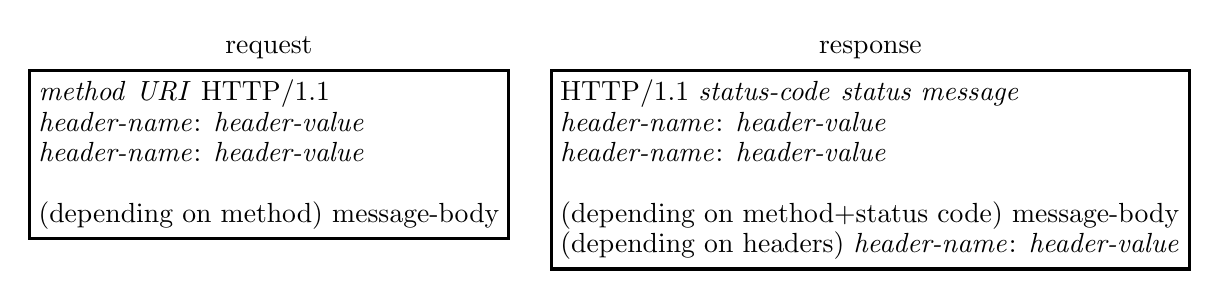
\begin{tikzpicture}
\node[draw,align=left,very thick,font=\fontsize{10}{11}\selectfont,label={north:request}] (request) {
\textit{method} \textit{URI} HTTP/1.1\\
\textit{header-name}: \textit{header-value} \\
\textit{header-name}: \textit{header-value} \\
~ \\
(depending on method) message-body
};
\node[anchor=north west,draw,align=left,font=\fontsize{10}{11}\selectfont,very thick,label={north:response}] 
at ([xshift=.5cm]request.north east){
HTTP/1.1 \textit{status-code} \textit{status message} \\
\textit{header-name}: \textit{header-value} \\
\textit{header-name}: \textit{header-value} \\
~ \\
(depending on method+status code) message-body \\
(depending on headers) \textit{header-name}: \textit{header-value}
};
\end{tikzpicture}